In order to perform a statistical interpretation, we have to prepare cards 
along with central and alternative shapes(histograms). The available tools \cite{lands}, \cite{combine}
do not take 2-dimensional histogram as an input, but 1-dimensional histograms
transformed from 2-dimensional ones. Since, the tools do nat care about 
how bins are arranged, we can unroll a 2-dimensional histogram to 1-dimensional one.

\begin{figure}[htp]
	\centering
	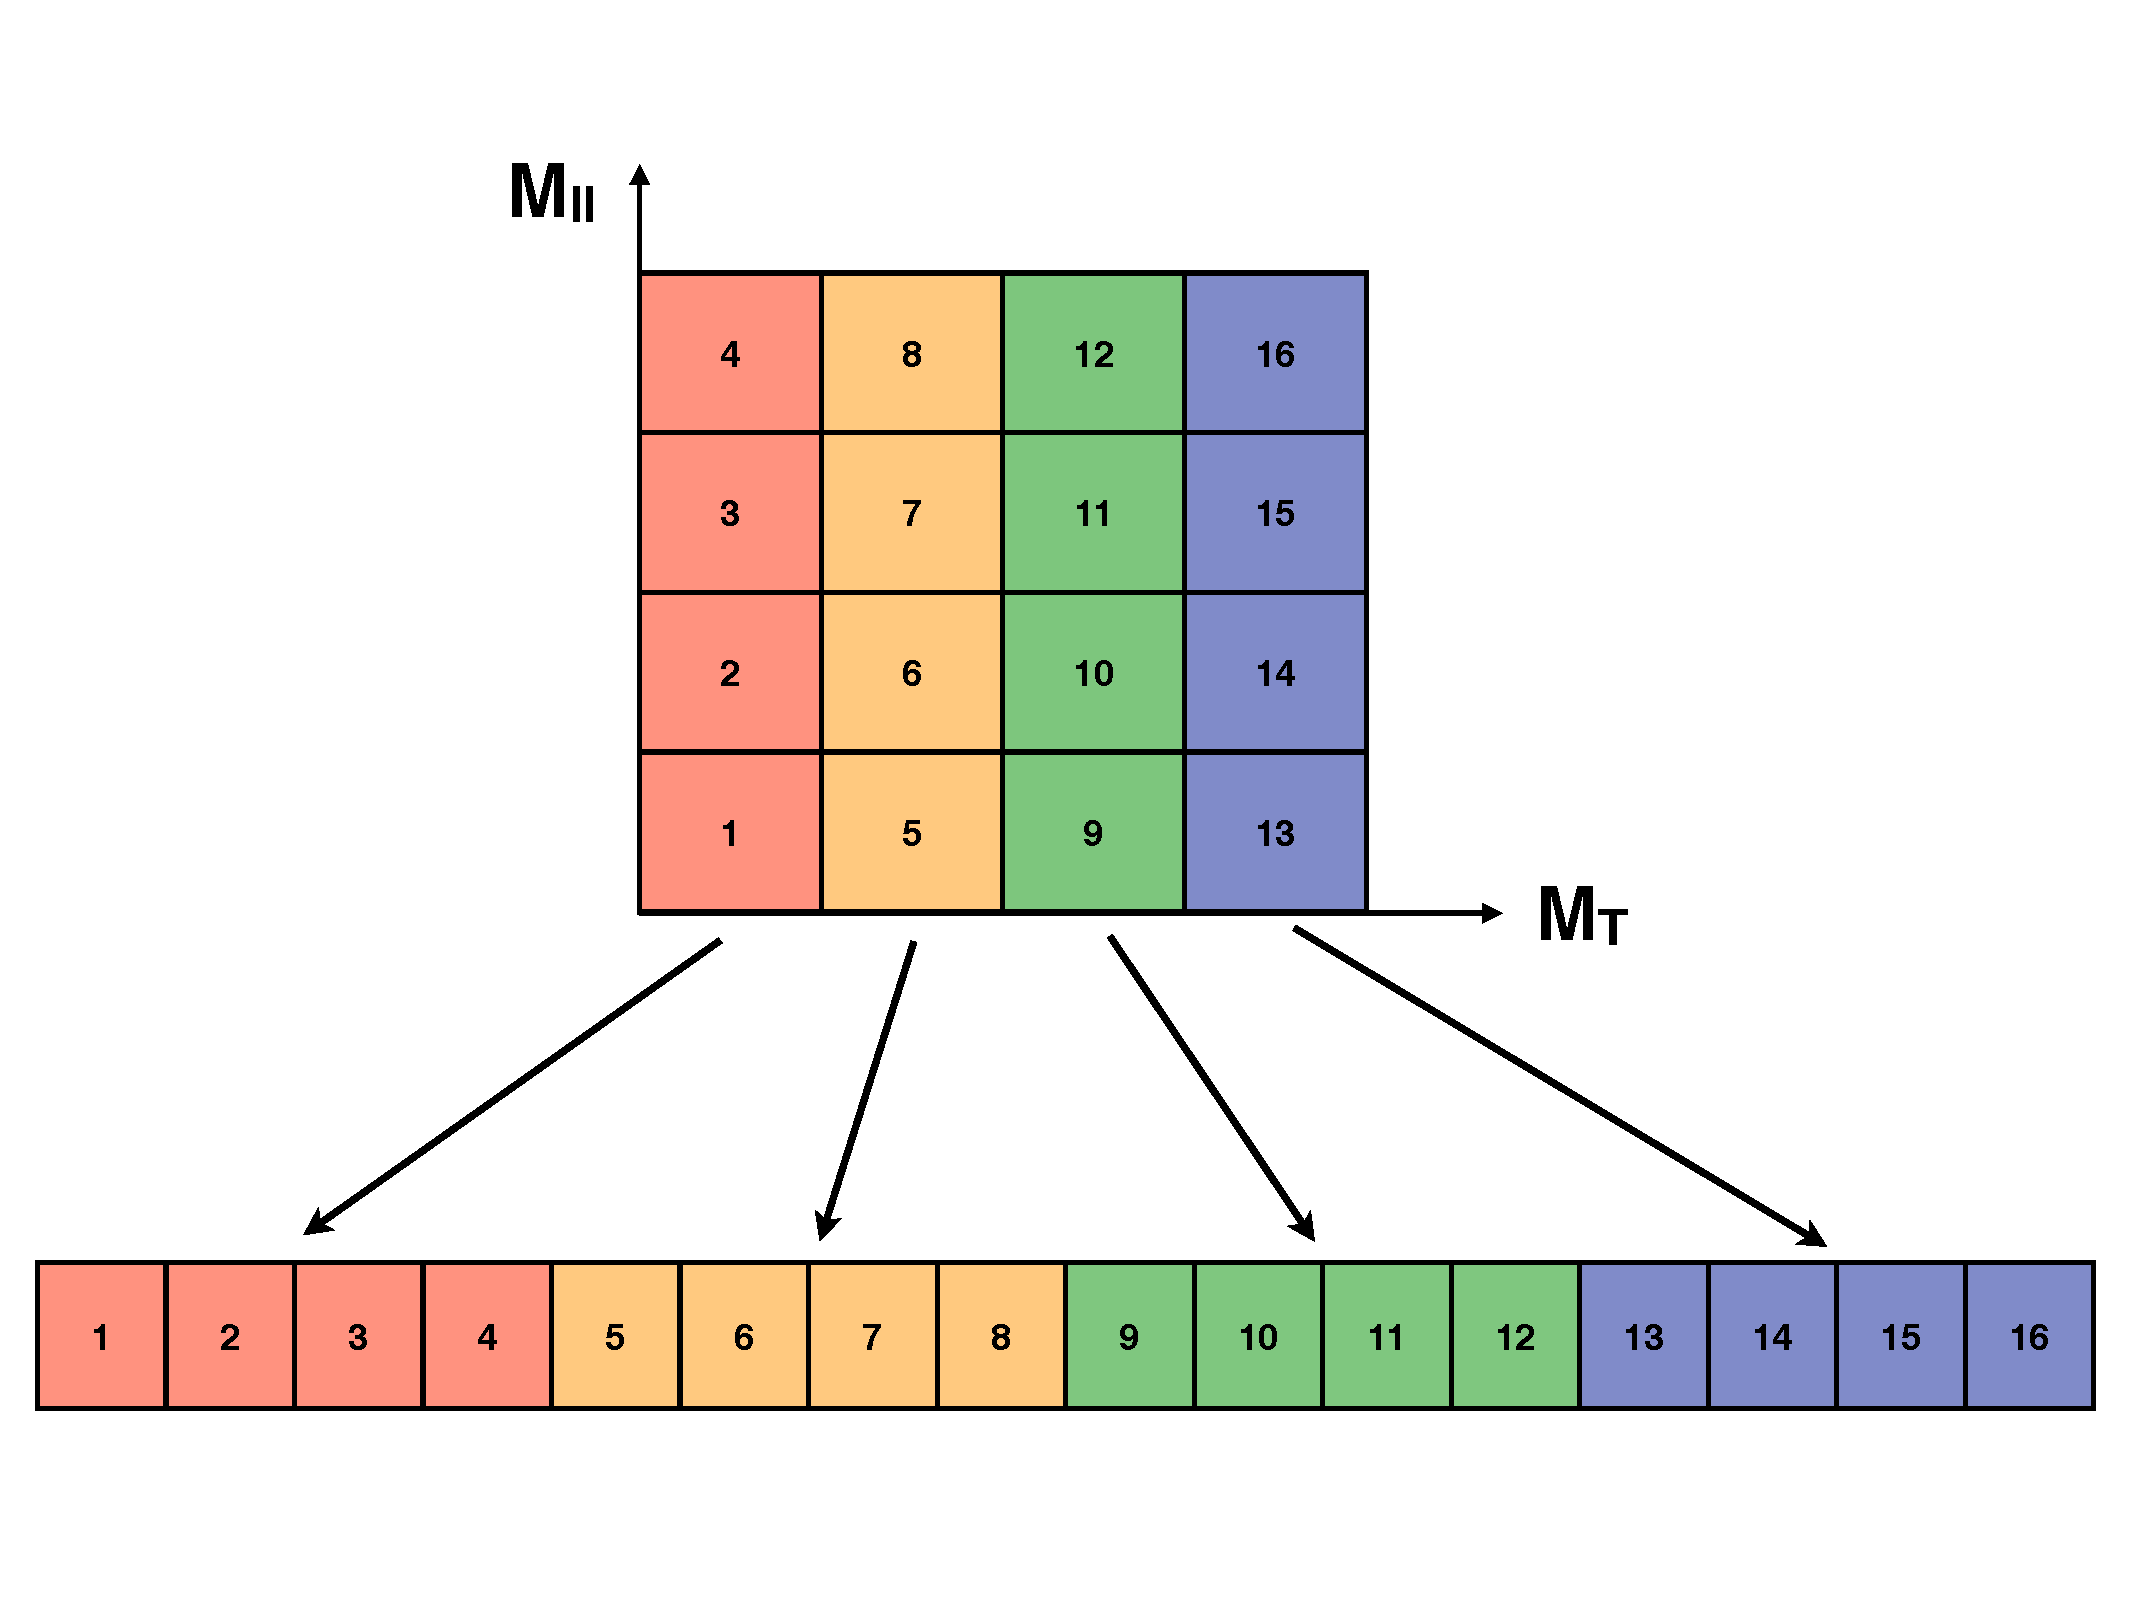
\includegraphics[width=0.8\textwidth]{figures/unrolling_schematic.pdf}
	\caption{ Schematic of how unrolling is done from 4x4 2D to 1D histogram. 
			  Same numbers in the 2D and 1D histograms indicates same bins.} 
  	\label{fig:unrolling_sch}
\end{figure}

Figure~\ref{fig:unrolling_sch} shows how unrolling is done for this study. 
In case of a 4x4 2D template, the first column in the 2D histogram 
becomes the 1st - 4th bins in the 1D histogram. The second column becomes 
5th - 8th bins in the 1D. Same thing goes until the last column.  

\begin{figure}[htp]
	\centering
	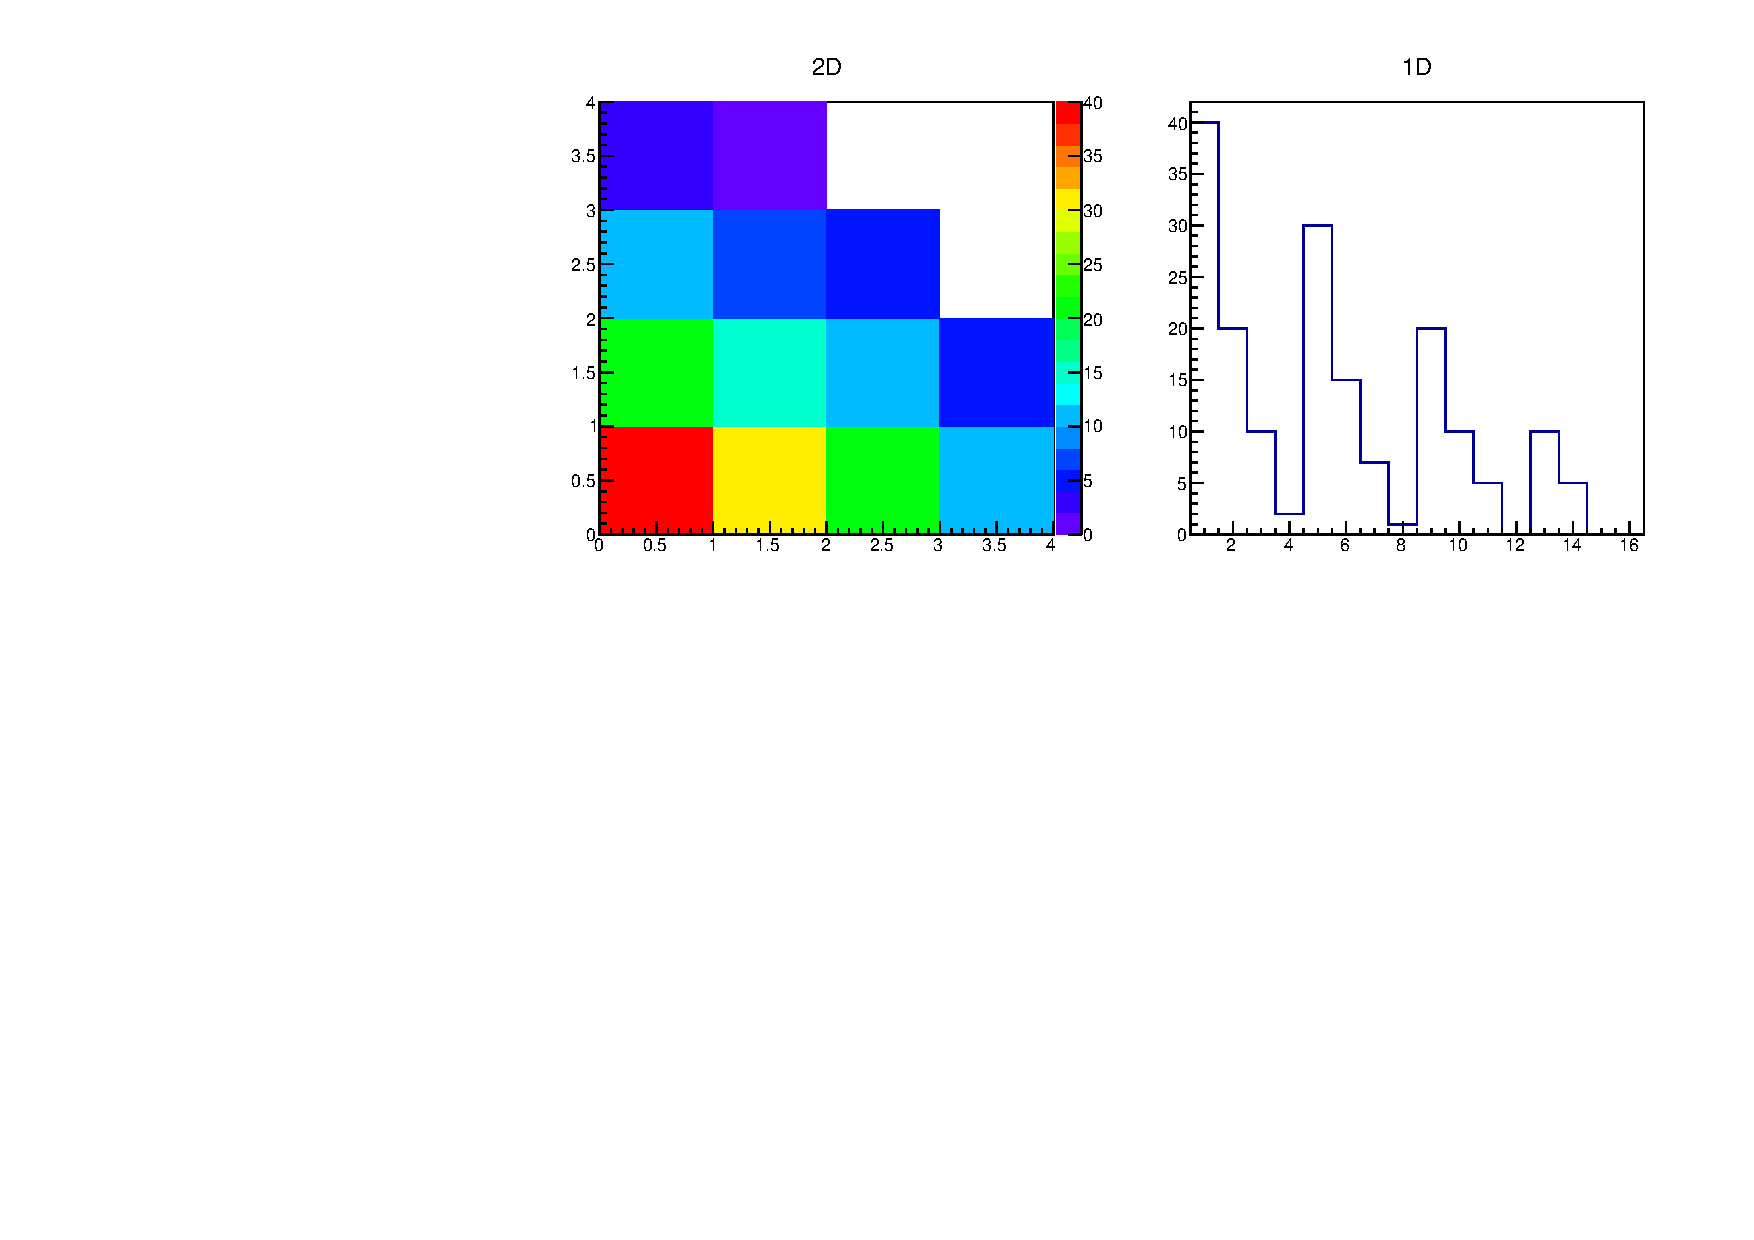
\includegraphics[width=0.8\textwidth]{figures/unrolling_example.pdf}
	\caption{ Example of how unrolling is done from 4x4 2D to 1D histogram.} 
  	\label{fig:unrolling_ex}
\end{figure}

Figure~\ref{fig:unrolling_ex} shows an example of 2D template and 
the corresponding unrolled template.  

On technical point of view, we can replace BDT template by unrolled 
template and run the same machinery.  

